\documentclass[oneside, 12pt]{book}

\usepackage{../_mypackages/mypreamble}
\usepackage[backend=biber,style=nature]{biblatex}
%\cite{barton} = [1] and \footfullcite[p. 324]{barton} = ^1 + footnote, p. 324 (e.g.)

\usepackage{../_mypackages/mycommands}
\usepackage{../_mythemes/mytheme1}

\addbibresource{ref_EM.bib}

%--------------------------------------------------------------



%--------------------------------------------------------------

\graphicspath{ {Electromagnetism/EM_figures/} }

\begin{document}
\pagestyle{mypage2}
\chapter{Optics}
\section{Monochromatic plane waves}
\begin{itemize}
    \item We have that the fields are the real parts of
    $$\tilde{\vb{E}}(\vb{r}, t) = \vb{E}_0e^{i(\vb{k}\vdot \vb{r} - \omega t)}\vu{e}_1$$
    $$\tilde{\vb{B}}(\vb{r}, t) = \frac{1}{v}\vb{E}_0e^{i(\vb{k}\vdot \vb{r} - \omega t)}(\vu{k}\cross \vu{e}_1) = \frac{1}{v}\vu{k} \cross \tilde{\vb{E}}$$
    where $\vb{k}$ is the propagation (or wave) vector and takes the forms
    $$k = \frac{2\pi}{\lambda} = \frac{2\pi \nu}{v} = \frac{\omega}{v}\qq{since} \omega = 2\pi \nu \qq{is the angular frequency of the wave}$$
    Then $v = 1/\sqrt{\mu \epsilon}$ is the wave speed in the media and $\epsilon$ and $\mu$ are the electric permeability  and magnetic permeability of the media, respectively. Remember that we'll be referring to the real parts of the complex fields above, which are sines and cosines.
    \item It is convenient to use the $\vb{H}$ vector, defined as
    $$\vb{H} = \frac{1}{\mu}\vb{B}$$
    hence
    $$H = \frac{E}{\mu v}$$
    and sometimes even the field $\vb{D}$, defined as
    $$\vb{D} = \epsilon \vb{E}$$
    hence
    $$D=\epsilon E$$
    \item The Poynting vector 
    $$\vb{S} = \vb{E}\cross\vb{H}$$
    is the directional energy flux density, whose units are
    $$[S] = \frac{J}{m^2-s}$$
    and for the case of monochromatic plane waves, it can be simplified to
    $$\vb{S} =\epsilon v E^2\ \vu{k}$$
    \item The energy density of the fields is
    $$u=\frac{1}{2}(\epsilon E^2 + \mu H^2)$$
    and for this case, it can be simplified to
    $$u= \epsilon E^2$$
    noting that the units are simply $$[u] = \frac{J}{m^3}$$
    \item Here we can see that the direction energy flux density is
    $$\vb{S} = vu\vu{k}$$
    \item Waves also carry momentum, in this case
    $$\vb{P} = \frac{u}{v}\vu{k}$$
    \item The average power per unit area transported by an electromagnetic wave is the intensity of the wave
    $$\vb{I} = \mean{\vb{S}} = \frac{1}{2}v\epsilon E_0^2\ \vu{k}$$
    and it isn't normally treated as a vector, but we'll be decomposing it into its perpendicular and parallel components to a surface.
    \end{itemize}
    
\section{Polarization}
\begin{itemize}
    \item The most general monochromatic plane wave is elliptically polarized. Supposing the wave vector is $\vu{k} = \vu{z}$ then the plane wave is on the $xy$-plane. The wave takes the following form
    $$E_x = Acos\left(kz-\omega t\right)$$
    $$E_y = Bcos\left(kz-\omega t + \delta \right)$$
    where $\delta$ is the phase difference between the components.
    \item For this generic plane wave, we can see how the components $E_x$ and $E_y$ relate by eliminating the term $kz-\omega t$. We achieve the following curve
    $$\left(\frac{E_x}{A}\right)^2 + \left(\frac{E_y}{B}\right)^2 - 2\left(\frac{E_x}{A}\right)\left(\frac{E_y}{B}\right)cos\delta = sin^2\delta$$
    \item We can have the linearly polarized wave if
    $$\delta = n\pi \qc n=0,\pm1, \pm2,...$$
    For $n$ even, we have
    $$\frac{E_y}{E_x} = \frac{B}{A}$$
    and for $n$ odd we have
    $$\frac{E_y}{E_x} = -\frac{B}{A}$$
    \begin{figure}[H]
        \centering
        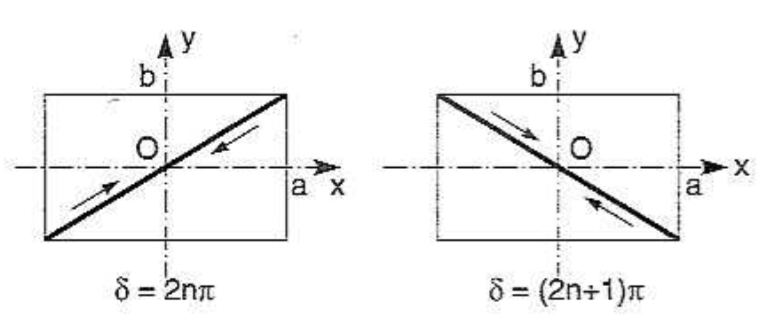
\includegraphics[width=\textwidth]{moyses4_fig_5-1}
    \end{figure}
    \item We can have the circularly polarized wave if
    $$A=B \qq{and} \delta =n\pi + \frac{\pi}{2}\qc n=0,\pm1,\pm2,...$$
    For even $n$, the rotation is counterclockwise, and if $n$ is odd, then the rotation is clockwise. On the complex plane the notation is
    $$E_x + iE_y = Ae^{i\omega t}\qq{for even} n$$
    and
    $$E_x + iE_y = Ae^{-i\omega t}\qq{for odd} n$$
    \item With the above result, we can see that we can write an arbitrary monochromatic plane wave as the superposition of two circularly polarized waves. Being
    $$\vu{\varepsilon}_+ = \frac{1}{\sqrt{2}}\left(\vu{x} + i\vu{y} \right)$$
    and
    $$\vu{\varepsilon}_- = \frac{1}{\sqrt{2}}\left(\vu{x} - i\vu{y} \right)$$
    we have that
    $$E_+ = Ae^{i(kz-\omega t)}\vu{\varepsilon}_+\qq{is counterclockwise}$$
    and
    $$E_- = Ae^{i(kz-\omega t)}\vu{\varepsilon}_-\qq{is clockwise}$$
    and hence we can write
    $$\vb{E} = \frac{1}{\sqrt{2}}\left(E_x-iE_y\right)\vu{\varepsilon}_+ +\frac{1}{\sqrt{2}}\left(E_x+iE_y\right)\vu{\varepsilon}_-$$
    This approach is useful for situations in which the refraction index depends on the direction of the circularly polarized wave (counterclockwise or clockwise).
\end{itemize}

\section{Reflection and transmission of waves}
\begin{itemize}
    \item The refraction index is defined as
    $$n = \frac{c}{v} = \frac{\sqrt{\mu \epsilon}}{\sqrt{\mu_ 0 \epsilon_0}}$$
    \item The situation is described on the figure below
    \begin{figure}[H]
    \centering
    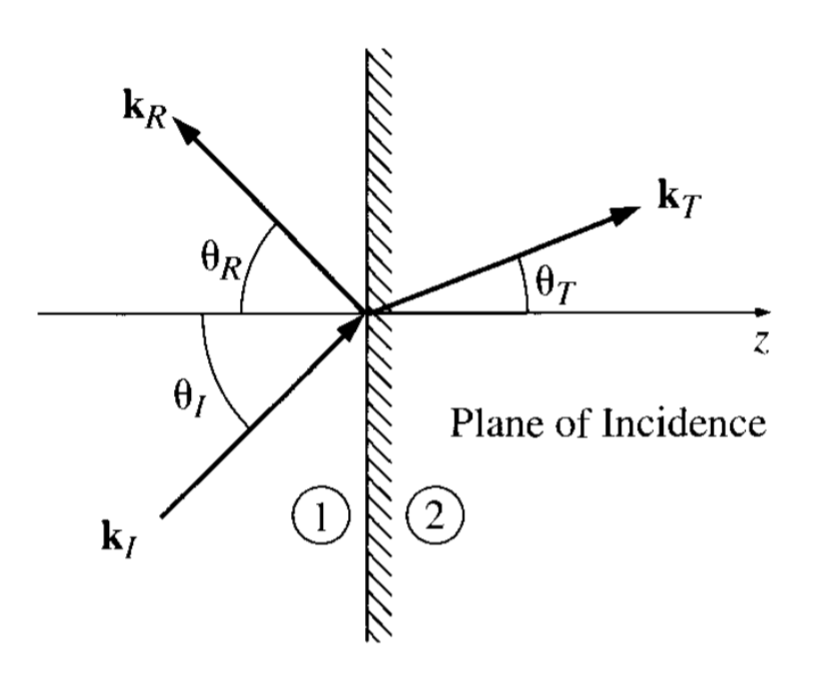
\includegraphics[width=0.7\textwidth]{griffithselectro_fig_9-14}
    \end{figure}
    where $I$, $R$ and $T$ refer to the incident, reflected and transmitted wave.
    \item It is important to note that all three waves have the same frequency $\omega$.
    \item There are three fundamental laws of geometrical optics, and they are
    \begin{enumerate}
        \item The incident, reflected and transmitted wave vectors form a plane (called the plane of incidence), which also includes the normal to the surface and the angle of incidence, the angle of reflection and the angle of transmission (of refraction) are all measured with respect to the normal.
        \item Law of reflection, which says that the angle of incidence is equal to the angle of reflection
        $$\theta_I = \theta_R$$
        \item Snell's law 
        $$n_1 sin\theta_I = n_2 sin\theta_T$$
    \end{enumerate}
    \item You'll have the three waves, and each of them can be decomposed into a perpendicular to the surface component and into a parallel to the surface component. The Fresnel's equations relate the amplitude of each of these components.
    \item The boundary condition at the surface of change of media can be derived from Maxwell's laws, and they are
    $$D_{I_{\perp}} + D_{R_{\perp}}= D_{T_{\perp}}$$
    $$E_{I_{\parallel}} + E_{R_{\parallel}} = E_{T_{\parallel}}$$
    $$B_{I_{\perp}} + B_{R_{\perp}} = B_{T_{\perp}}$$
    $$H_{I_{\parallel}} + H_{R_{\parallel}} = H_{T_{\parallel}}$$
    where $D_{I_{\perp}}$ is the perpendicular component of the incident $D$ field, for example.
    \item The boundary conditions result in the Fresnel's equations
    $$\frac{E_{R_{\parallel}}}{E_{I_{\parallel}}} = \frac{(n_1/\mu_1)cos\theta_T - (n_2/\mu_2)cos\theta_I}{(n_1/\mu_1)cos\theta_T + (n_2/\mu_2)cos\theta_I}$$
    $$\frac{E_{R_{\perp}}}{E_{I_{\perp}}} = \frac{(n_1/\mu_1)cos\theta_I - (n_2/\mu_2)cos\theta_T}{(n_1/\mu_1)cos\theta_I + (n_2/\mu_2)cos\theta_T}$$
    $$\frac{E_{T_{\parallel}}}{E_{I_{\parallel}}}  = \frac{2(n_1/\mu_1)cos\theta_I}{(n_1/\mu_1)cos\theta_T + (n_2/\mu_2)cos\theta_I}$$
    $$\frac{E_{T_{\perp}}}{E_{I_{\perp}}} = \frac{2(n_1/\mu_1)cos\theta_I}{(n_2/\mu_2)cos\theta_I + (n_1/\mu_1)cos\theta_T}$$
    where $E_{R_{\parallel}}$ is the parallel component of the electric field of the reflected wave, for example. We this, you can construct the resulting waves. For example, the total amplitude of the reflected wave is $E_R^2 = E_{R_{\parallel}}^2 + E_{R_{\perp}}^2$.
    \item If $\mu_1 = \mu_2 = \mu$, using Snell's law we can write
    $$\frac{E_{R_{\parallel}}}{E_{I_{\parallel}}} = -\frac{tan(\theta_I - \theta_T)}{tan(\theta_I + \theta_T)}$$
    $$\frac{E_{R_{\perp}}}{E_{I_{\perp}}} = -\frac{sin(\theta_I - \theta_T)}{sin(\theta_I + \theta_T)}$$
    $$\frac{E_{T_{\parallel}}}{E_{I_{\parallel}}} = \frac{2sin\theta_I\theta_T}{sin(\theta_I + \theta_T)cos(\theta_I - \theta_T)}$$
    $$\frac{E_{T_{\perp}}}{E_{I_{\perp}}} = \frac{2sin\theta_I\theta_T}{sin(\theta_I + \theta_T)}$$
    \item Relating the intensity of the waves, we have that
    $$I_I = \frac{1}{2}\epsilon_1 v_1 E_I^2 cos\theta_I$$
    $$I_R = \frac{1}{2}\epsilon_1 v_1 E_R^2 cos\theta_I$$
    $$I_T = \frac{1}{2}\epsilon_2 v_2 E_T^2 cos\theta_T$$
    noting that the cosines appear because we are looking at the intensity that gets to the surface, so we don't look the intensity parallel to it, we look only at the perpendicular intensity.
    \item We define the reflection coefficient as
    $$R = \frac{E_R}{R_I}$$
    \item We define the transmission coefficient as
    $$T = \frac{E_T}{E_I}$$
\end{itemize}

\end{document}